% Compile from the manuscript directory with graphicx loaded.
\begin{figure*}[t]
  \centering
  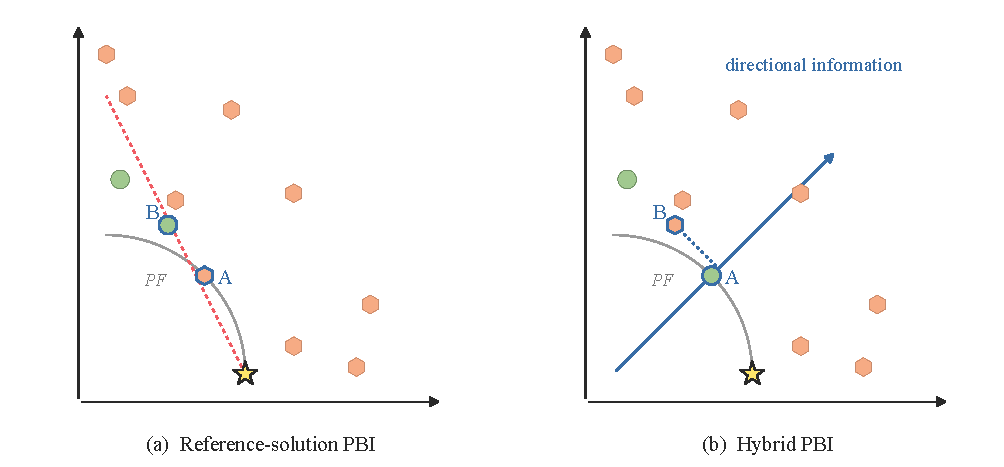
\includegraphics[width=170mm]{figures/paqc_correction_simple/paqc_simple_en.pdf}
  \caption{Grouping by reference-solution PBI and hybrid PBI.
  The star denotes the prescribed reference, circles and hexagons denote the
  positive and non-positive groups, and the gray curve is the known Pareto front.
  (a) Reference-based classification excludes $A$ on the front and includes $B$
  outside it. (b) With directional scoring, $A$ enters the positive group while
  $B$ is excluded. The blue arrow and dotted segment indicate the associated
  direction and $B$'s perpendicular distance. Both panels use identical
  coordinates. This constructed example prescribes one reference, three
  uniform directions, and budget progress $t=0.20$; the known front is not
  used for scoring.}
  \label{fig:paqc-simple-correction}
\end{figure*}
